\documentclass[11pt]{article}
\usepackage{amsmath}
\usepackage{fancyhdr}
\usepackage{hyperref}
\usepackage{graphicx}
\newcommand{\compactlist}{\setlength{\itemsep}{0pt} \setlength{\parskip}{0pt} \setlength{\leftskip}{-1em}}
\usepackage[top=0.9in, bottom=0.8in, left=0.9in, right=0.9in]{geometry}

\lhead{MATH 4263/5373}
\rhead{Sep. 10, 2019}
\chead[RE]{Fixed-point iterations: II}
\cfoot{}
\rfoot{}%Code for figure and report is (not yet) available in the class folder.}
\pagestyle{fancy}

\begin{document}

Consider the root-finding problem \(f(x) = x^4-3x^2-3\). It has many different, but equivalent, fixed-point problems.
\begin{align*}
g_1(x) & = x- f(x) = x\\
g_2(x) & = x+f(x) = x\\
g_3(x) & = \sqrt{\frac{3}{x^2-3}} = x\\
g_4(x) & = x - \frac{x^4-3x^2-3}{4x^3-6x}
\end{align*}

%\begin{figure}[h!]
\begin{center}
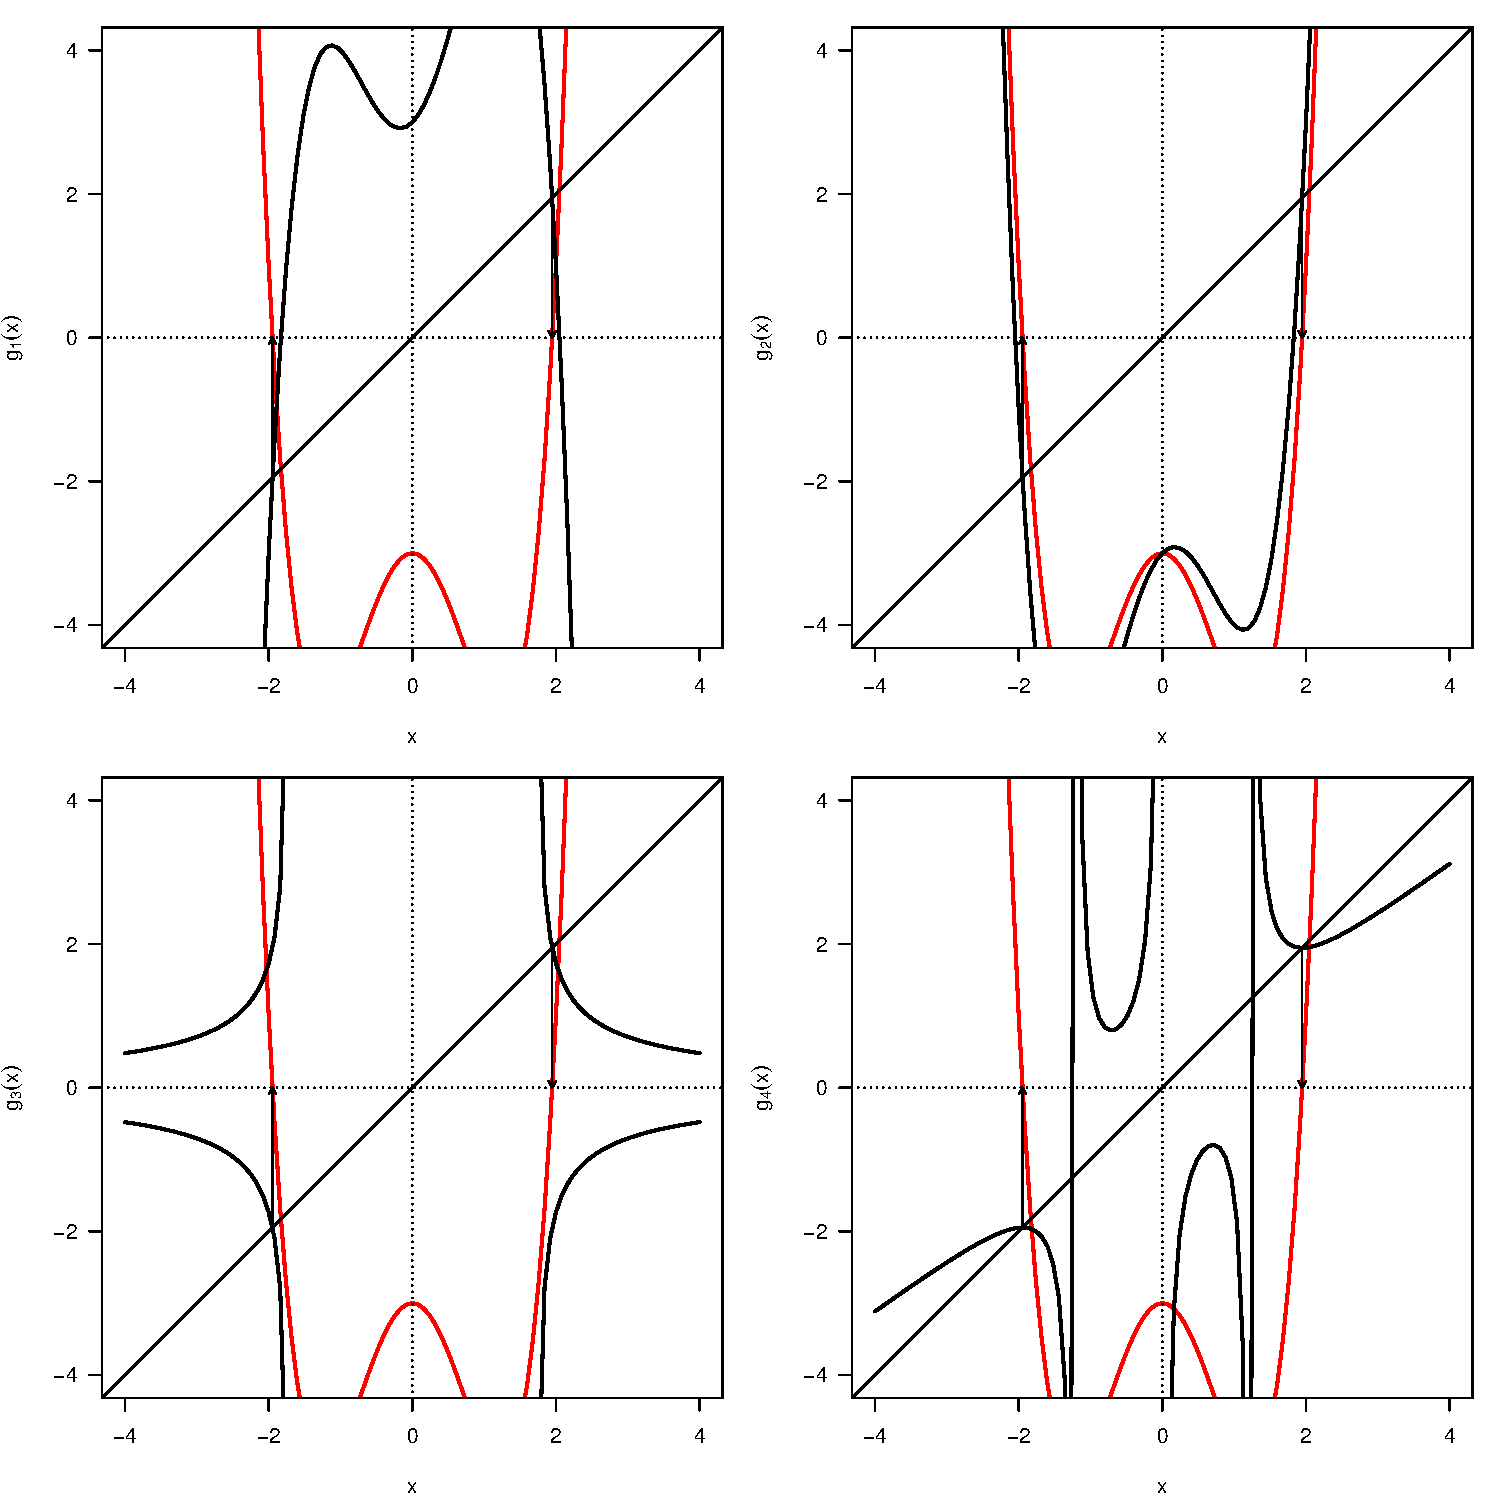
\includegraphics[width=\textwidth]{bad.pdf}
\end{center}
%\caption{Two functions that give rise to fixed-point problems. Dotted corresponds to the negative value of the square root and the solid line corresponds to the positive value. Left: intersections of each with the black \(1:1\) line indicate fixed points. Right: values between \(-1\) and \(1\) indicate that a fixed point, if it exists, is unique.}\label{fig::g1}
%\end{figure}

\newpage
A better formulation is given by \[g_5(x) = \sqrt[4]{3x^2+3}\]

%\begin{figure}[h!]
%\begin{minipage}{0.48\textwidth}
\begin{center}
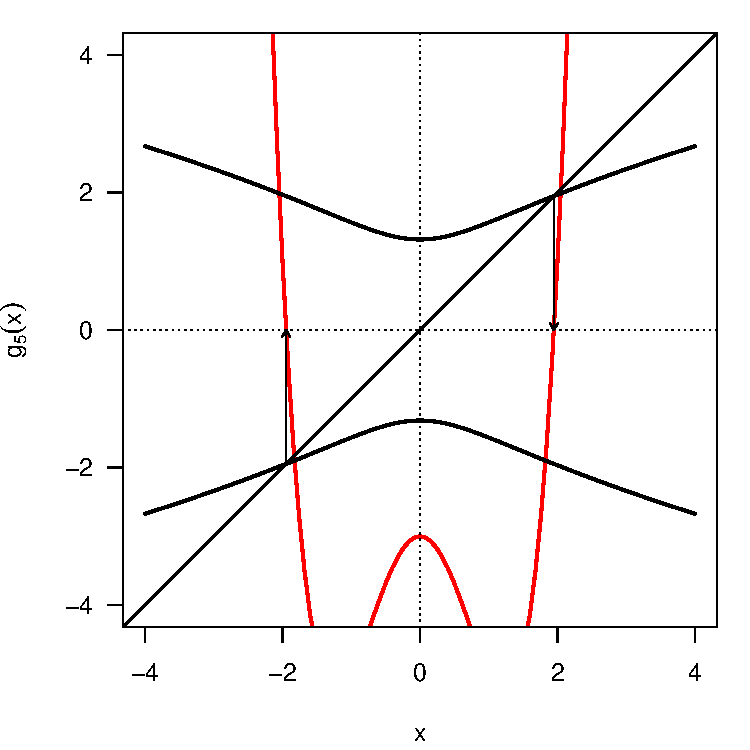
\includegraphics[width=0.5\textwidth]{good.pdf}
\end{center}%\end{minipage}
%\begin{minipage}{0.48\textwidth}
%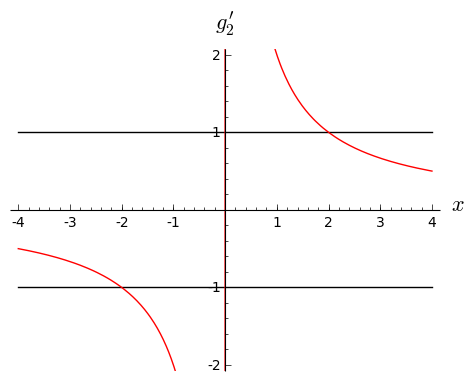
\includegraphics[width=\textwidth]{g2p.png}
%\end{minipage}
%\caption{Left: intersections with the black \(1:1\) line indicate fixed points. Right: values between \(-1\) and \(1\) indicate that a fixed point, if it exists, is unique. Notice that the smaller the value of the fixed point, the steeper the function \(g_2(x)\).}\label{fig::g2}
%\end{figure}


\end{document}














